\chapter{Pierre Auger Observatory}\label{Ch:PAO}


Science Goals of the Pierre Auger Observatory is to probe the origins and characteristics of cosmic rays above 10$^{17}$ eV and to study the interactions of the most energetic particles observed in nature.

The Pierre Auger Observatory (PAO) is an hybrid detector that is located near Malarg\"ue in the Mendoza Province, Argentina. PAO consists of 1660 Cherenkov water detector spread over 3000 km$^2$  by 24 fluorescence telescopes. 

\begin{figure}[hp]
\centering
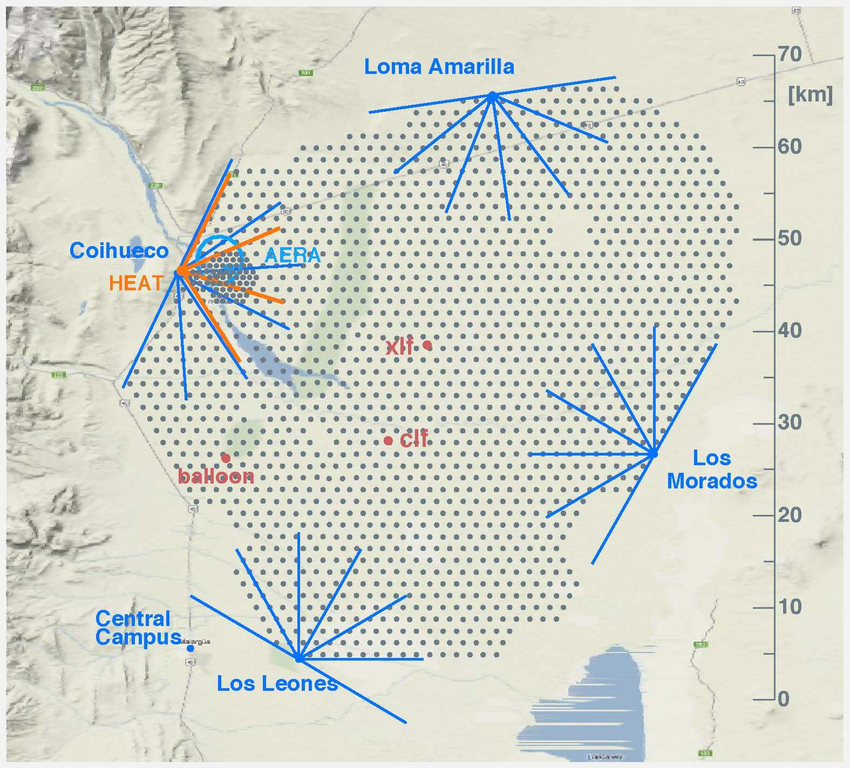
\includegraphics[width=0.7\textwidth]{chapters/pix/PAO_equipment_layout_overview.png}
\caption{Image of layout of Pierre Auger Observatory located near Malargue, Argentina.}
\label{fig:PAO_layout}
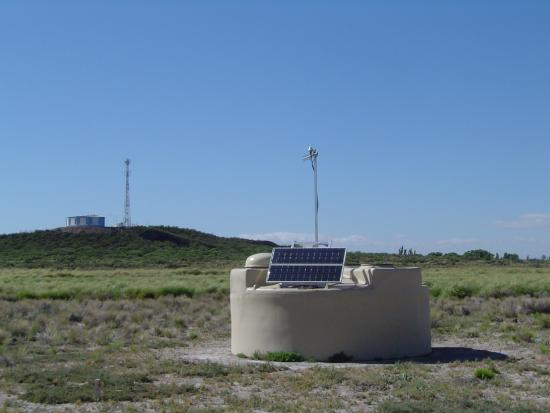
\includegraphics[width=0.7\textwidth]{chapters/pix/pierre-auger-observatory_tankAndTelescope.jpg}
\caption{Image of one of the fluorescence detector site (background) and one of the surface detectors (foreground).}
\label{fig:PAO_TankAndTelescope}
\end{figure}


\section{Surface Detector}

\begin{figure}
\centering
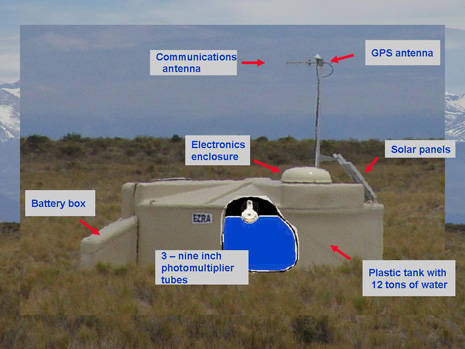
\includegraphics[width=0.7\textwidth]{chapters/pix/inside_surface_detector.jpg}
\caption{Basic schematic of a surface detector.}
\label{fig:SD_schematic}
\end{figure}

\section{Fluorescence Detector}

\begin{figure}
\centering
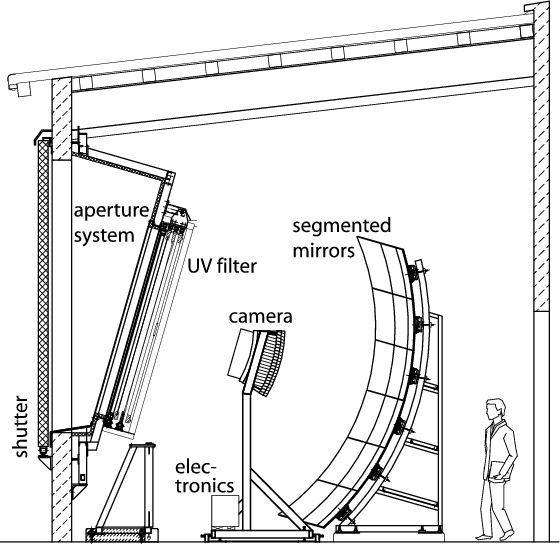
\includegraphics[width=0.7\textwidth]{chapters/pix/fluorescence_telescope.png}
\caption{Basic schematic of a fluorescence telescope.}
\label{fig:FD_schematic}
\end{figure}

\subsection{Photomultiplier Tubes}

\section{Communication System and CDAS}

\section{Event Reconstruction}

\subsection{Surface Detector}

\subsection{Fluorescence Detector}

\section{Enhancements and future upgrades}